\chapter{Medical Imaging and Image Segmentation}
%

The first steps in image-based modeling and simulation involve \textit{image acquisition}, \textit{image processing}, and \textit{image segmentation}. Several techniques are available to produce three-dimensional image data of an anatomical region of interest and are reviewed herein. State-of-the art image processing and image segmentation approaches are summarized in this section as well.

%%%%%%%%%%%%%%%%%%%%%%%%%%%%%%%%%%%%%%%%%%%%%%%
%%%%%%%%%%%%%%%%%%%%%%%%%%%%%%%%%%%%%%%%%%%%%%%
\section{Imaging Approaches}
\label{Imaging Approaches}

Medical imaging is the process of generating discrete image representations of biological tissues. Of the many imaging modalities found in clinical and research settings, the most prevalent are \textit{magnetic resonance imaging} (MRI) and \textit{x-ray computed tomography} (CT). Both approaches are \textit{tomographic} in that they produce a series of two-dimensional images representing thin slices through the region, that are subsequently combined to produce a three-dimensional volume representation \cite{larobina_murino_2014}. The data measured during acquisition are different for each modality, and thus the use case typically governs which technique is most appropriate. Images typically have resolutions on the order of millimeter or sub-millimeter resolution. Several other imaging techniques exist - some of which provide more information than do MRI and CT - and are briefly presented in this section as well. Finally, typical data storage and file formats are discussed.

\subsection{Magnetic Resonance Imaging}
\label{Magnetic Resonance Imaging}

Magnetic resonance imaging (MRI) is the process of generating images via the physical phenomenon of nuclear magnetic resonance (NMR), in which nuclei in a magnetic field absorb and re-emit electromagnetic radiation at their \textit{resonant frequency}~\cite{NMR}. Gradients in the magnetic field are used to encode the response at different locations in the region. MRI provides excellent soft tissue contrast, for tissues such as articular cartilage, bone marrow, muscle, ligaments, and gray and white matter in the brain. Unlike CT, it does not use any harmful ionizing radiation~\cite{waldman_campbell}. A brief description of the basic physics in acquiring an MRI follows.

A strong external magnet generates a magnetic field $B_0\bm{e}_z$ that is constant in time and space, within which the patient or object is placed. For most clinical applications, the strength of this field is 1.5 Tesla or 3 Tesla. The $z$ direction corresponds to the image slice thickness direction. Shim coils are used to correct or "shim" the magnetic field so as to ensure good field homogeneity, which results in a high-quality signal~\cite{jacobs_2007}. Dipole moments in the nuclei of certain elements align either in parallel or anti-parallel to the direction of the applied magnetic field, similarly to how a bar magnet orients itself in the presence of an external magnetic field~\cite{hendrick_1994}. The parallel orientation provides a slightly lower energy state than that for the anti-parallel orientation, and thus the dipole moments prefer to align with the direction of the applied magnetic field. Prior to applying the external magnetic field, the random orientation of the nuclear magnetic dipoles in the tissue produce a zero net magnetization. Following the imposition of a static magnetic field, a net magnetization of tissue $M_0\bm{e}_z$ is produced from the preferential alignment of dipoles. See \figref{mr1}.

Due to the prevalence of hydrogen in biological tissues - most notably in water and fat - MR imaging is typically based on the behavior of the nuclear magnetic dipole of hydrogen.

\begin{figure}[ht]
\centering
\subfigure[]{%
		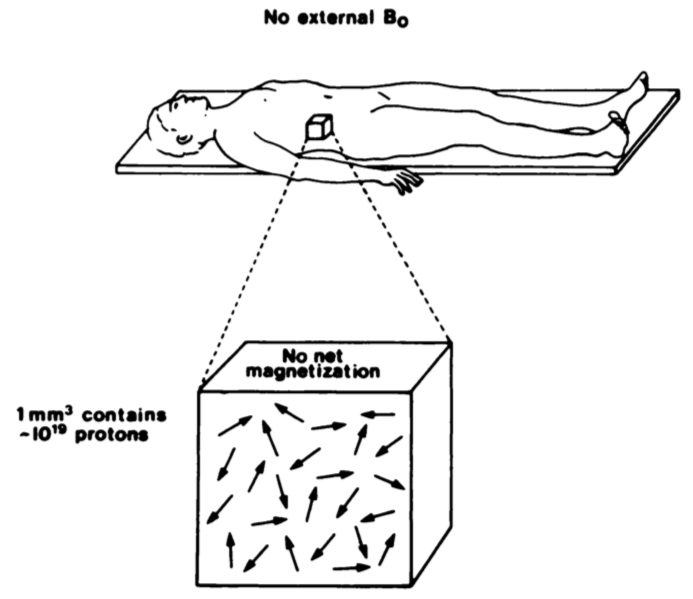
\includegraphics[scale=0.33]{media/0-imaging/mr1a.png}
\label{fig:mr11}}
\subfigure[]{%
		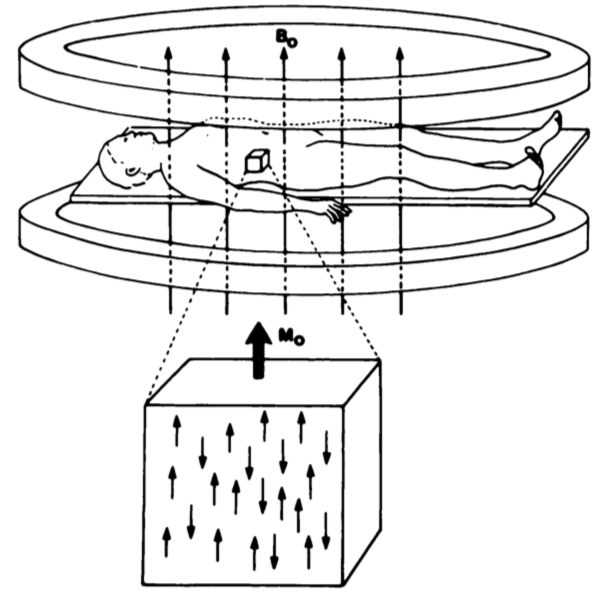
\includegraphics[scale=0.33]{media/0-imaging/mr1b.png}
\label{fig:mr12}}
%
\caption{Net magnetization $M_0$ in a voxel of tissue (a) prior to, and (b) following the application of a static external magnetic field $B_0$~\cite{hendrick_1994}}
\label{fig:mr1}
\end{figure}

If the net magnetization is perturbed from pointing in the same direction of a magnetic field $B\bm{e}_z$, the new magnetization $M$ \textit{precesses} about the $z$ axis. The \textit{precessional frequency} or \textit{Larmor frequency} $\omega$ is defined by the following relationship:
\begin{equation}
\omega = \gamma B
\end{equation}
where the constant $\gamma$ is the \textit{gyromagnetic ratio}, which is 42.6 MHz/T for hydrogen. In MR imaging, the net magnetization is tipped away from the direction of $B_0$ by applying a radio-frequency (RF) pulse that oscillates exactly at the Larmor frequency. The precessing transverse magnetization produces a changing magnetic field, which induces an electric current and is recorded by the receiver coil. See \figref{mr2}.

\begin{figure}[ht]
\centering
\subfigure[]{%
		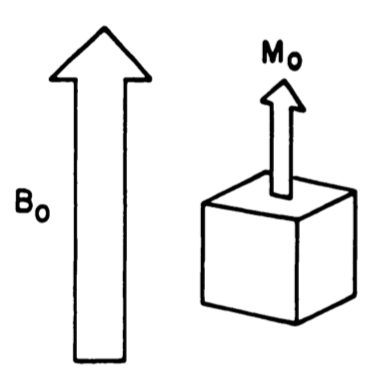
\includegraphics[scale=0.25]{media/0-imaging/mr2a.png}
\label{fig:mr21}}
\subfigure[]{%
		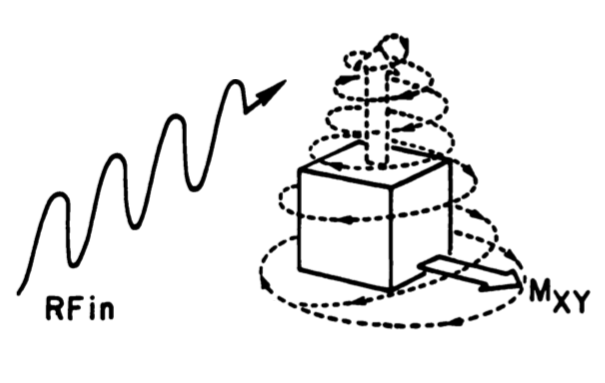
\includegraphics[scale=0.25]{media/0-imaging/mr2b.png}
\label{fig:mr22}}
\subfigure[]{%
		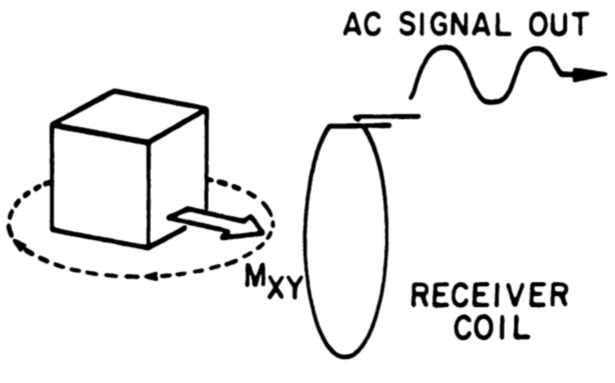
\includegraphics[scale=0.25]{media/0-imaging/mr2c.png}
\label{fig:mr23}}
%
\caption{Basic premise of MRI: (a) An external magnetic field $B_0$ causes net magnetization $M_0$ of a voxel of tissue pointing in the same direction as the applied field, (b) an RF pulse applied at the precessional frequency of hydrogen causes the magnetization vector to tilt from a longitudinal direction into the transverse plane, and (c) the amplitude, frequency, and phase of the time-varying signal from the transverse magnetization $M_{xy}$ is recorded~\cite{hendrick_1994}}
\label{fig:mr2}
\end{figure}

In order for the receiver coil to distinguish between different locations in the object, \textit{spatial localization} of the MR signal is achieved by applying linear magnetic field gradients in each of the three spatial directions. Namely, the new spatially varying magnetic field $B(\bm{x})\bm{e}_z$ (still pointing in $z$ direction), following the imposition of magnetic gradients, becomes:
\begin{equation}
B(\bm{x}) = B_0 + \bm{G}(t) \cdot \bm{x}
\label{eqn:gradient}
\end{equation}
The magnetic field gradient $\bm{G}(t) = (G_x, G_y, G_z)$ is applied in stages, to be discussed shortly. Multiplying \eqnref{gradient} by $\gamma$ yields:
\begin{equation}
\omega(\bm{x}) = \omega_0 + \bm{G}(t) \cdot \bm{x}
\label{eqn:freq}
\end{equation}
Thus, each RF signal oscillates at the appropriate frequency to excite and record information for each unique voxel in the image. Specifically, the magnetic gradient $G_z$ and corresponding RF pulse are first turned on to excite a particular slice (or section) of tissue. Excitation here refers to the perturbation of the net magnetization from the $z$ direction into the transverse plane. $G_z$ is referred to as the \textit{slice-selection gradient}. The resolution of the image in the $z$ direction may be increased by reducing the bandwidth of the RF pulse or increasing the strength of the applied gradient.

To resolve the selected section into voxels, gradients are applied separately in each of the two in-plane directions $x$ and $y$. The magnetic gradient $G_y$ is applied and removed following signal excitation and before signal measurement. While turned on, the gradient causes strips of hydrogen nuclei within the slice to precess at different speeds for a brief period of time. When the gradient is turned off, different strips maintain the same precessional frequency within the same slice, but a fixed phase difference now exists among them. $G_y$ is referred to as the \textit{phase-encoding gradient}. Finally, the magnetic gradient $G_x$ alters the resonant frequency along the $x$ direction. It separates each strip into voxels, each voxel resonating at a different frequency. $G_x$ is applied at the time of signal measurement and is referred to as the  \textit{frequency-encoding gradient} or the \textit{readout gradient}. The resolution of the in-plane image may be increased by increasing the number of pulse sequence acquisitions and subsequent measurements. See \figref{mr3} for a visual representation of these steps.

\begin{figure}[ht]
\centering
\subfigure[]{%
		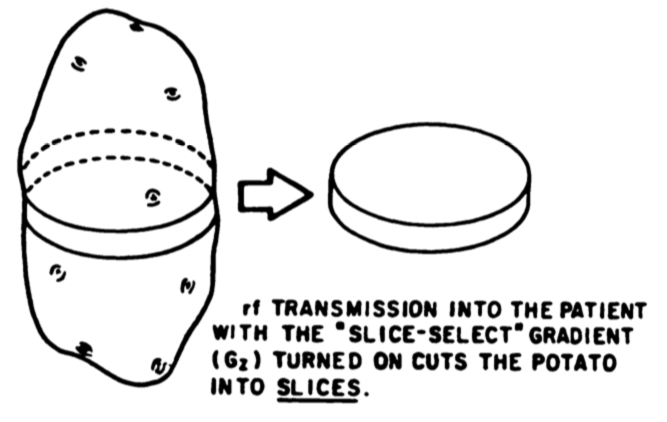
\includegraphics[scale=0.21]{media/0-imaging/mr3a.png}
\label{fig:mr31}}
\subfigure[]{%
		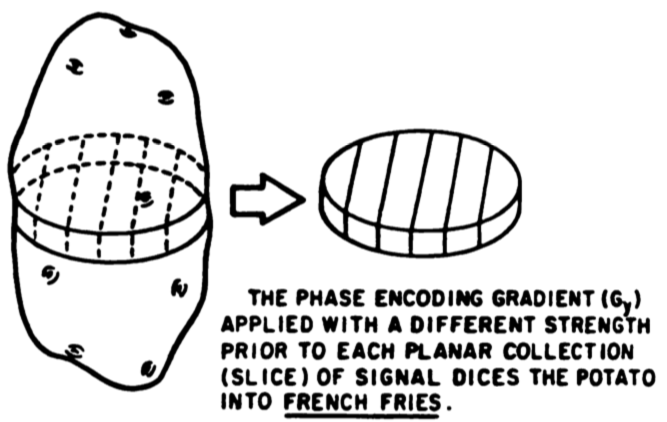
\includegraphics[scale=0.21]{media/0-imaging/mr3b.png}
\label{fig:mr32}}
\subfigure[]{%
		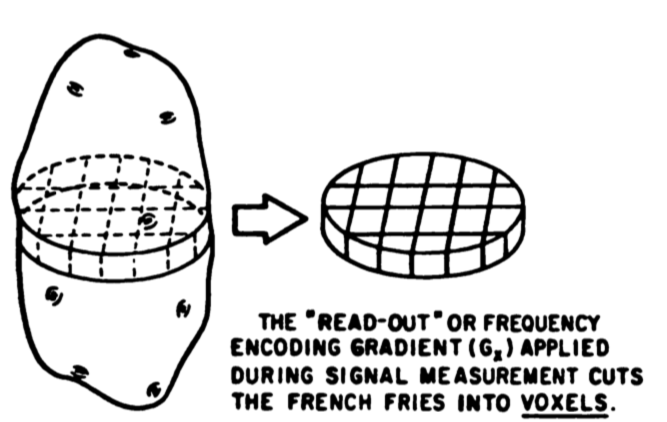
\includegraphics[scale=0.21]{media/0-imaging/mr3c.png}
\label{fig:mr33}}
%
\caption{Visual representation of the process of spatial localization based on successive application of magnetic gradients: (a) slice-selection gradient, (b) phase-encoding gradient, and (c) frequency-encoding gradient~\cite{hendrick_1994}}
\label{fig:mr3}
\end{figure}

MRI signal intensity at a particular voxel typically depends on the proton density of the tissue (via the strength of the net magnetization $M_0$) and two \textit{relaxation times} T1 and T2 corresponding to the exponential decay of the perturbed net magnetization back to its original state following an RF pulse. Following a typical $90^{\circ}$ RF pulse, which maximizes the transverse magnetization $M_{xy}$, the relaxation times are defined as such:
\begin{equation}
M(t) = M_0(1 - e^{(-t/T1)})
\end{equation}
\begin{equation}
M_{xy}(t) = M_{xy}e^{(-t/T2)}
\end{equation}
The \textit{spin-lattice}, \textit{longitudinal}, or \textit{T1 recovery time} corresponds to the recovery of the longitudinal magnetization $M_0$. This reorientation is caused by the transfer of energy from the excited magnetic dipoles to the surrounding lattice of molecules. The \textit{transverse}, \textit{spin-spin}, or \textit{T2 recovery time} corresponds to neighboring precessing magnetic dipoles \textit{dephasing}. Dephasing is caused by different magnetic environments for different hydrogen nuclei within the same voxel as the transverse magnetization decays.

Tissue contrasts are created based on the strength and timing of the RF pulse; this is known as the \textit{MR sequence}. The parameters in MR pulse sequences weight the influence of proton density, T1, and T2 differently in the final MR signal. The most basic MR sequences are \textit{proton density} (PD), \textit{T1-weighted} (T1W), and \textit{T2-weighted} (T2W), each of which provide different tissue contrasts. The choice of an MR sequence will depend on the tissues and applications of interest of the scan. A number of references are available  \cite{nishimura_2010, brown_semelka_2003, webb_2003} for a more detailed description of T1, T2, the parameters of an MR sequence, and their relationship in creating tissue contrast.

For each voxel in a slice, the amplitude, phase, and frequency of the time-varying MR signal is recorded by the receiver coil in the \textit{frequency domain}, or what is known as \textit{k-space}. For each slice, the frequency domain is converted to the spatial domain (i.e., the two-dimensional image for a particular slice) via 2D inverse Fourier transform. The k-space of an image can be modified to identify artifacts, remove noise, and enhance contrast~\cite{imaios}. Please refer to the references in this section for more detail on k-space and its manipulations. Finally, each 2D image is combined to form a 3D grayscale image corresponding to the object scanned. The intensity at each voxel in the three-dimensional rectilinear grid is a weighted proton density. The value at each voxel can represent many different units of measure depending on the pulse sequence~\cite{beek_hoffman_2008}.

\subsection{X-Ray Computed Tomography}
\label{X-Ray Computed Tomography}

X-ray computed tomography (CT) is the process of generating images via the emission an x-ray beam source, and subsequently detecting the \textit{attenuation} of the x-ray beam through the various tissues in the patient or object. CT provides excellent contrast for bone, but is less suitable in measuring soft tissue contrast compared to MRI. Acquisition times are typically less than those for MRI, image resolutions are typically higher~\cite{pomeranz_2007}, and ionizing radiation from the x-ray beam must be carefully considered. The basic principles of image acquisition via CT technology ensues.

In CT, an x-ray beam source is emitted through the plane of a finite thickness cross section of the object~\cite{mahesh_2002}. The mean attenuation of the x-ray beam through each voxel within the slice is measured by a detector on the other side of the object. The attenuation data is reconstructed into a digital two-dimensional image. Once again, the set of 2D images is stacked together to form a 3D image representation of the region being scanned.

Attenuation measures the amount by which x-ray radiation is reduced in passing through material. For an inhomogeneous material, the attenuation along a particular ray line is expressed in the following relationship:
\begin{equation}
I= I_0e^{-\int\limits_{0}^{L}f(x,y) ds}
\label{eqn:init}
\end{equation}
where $I_0$ is the x-ray intensity emitted in front of the object, $I$ is the x-ray intensity received behind the object, $f(x,y)$ is the linear attenuation coefficient for the material at location $(x,y)$, and $L$ is the length over which the beam travels though the material, and $ds$ is the length of a differential cut along the ray. The variable $s$ is parameterized as a function of $x$ and $y$. In first generation CT machines, for a particular slice, the x-ray tube and detector were rigidly translated together across the subject as x-ray beams were emitted and recorded~(\figref{ct1}).

\begin{figure}[ht]
\centering
		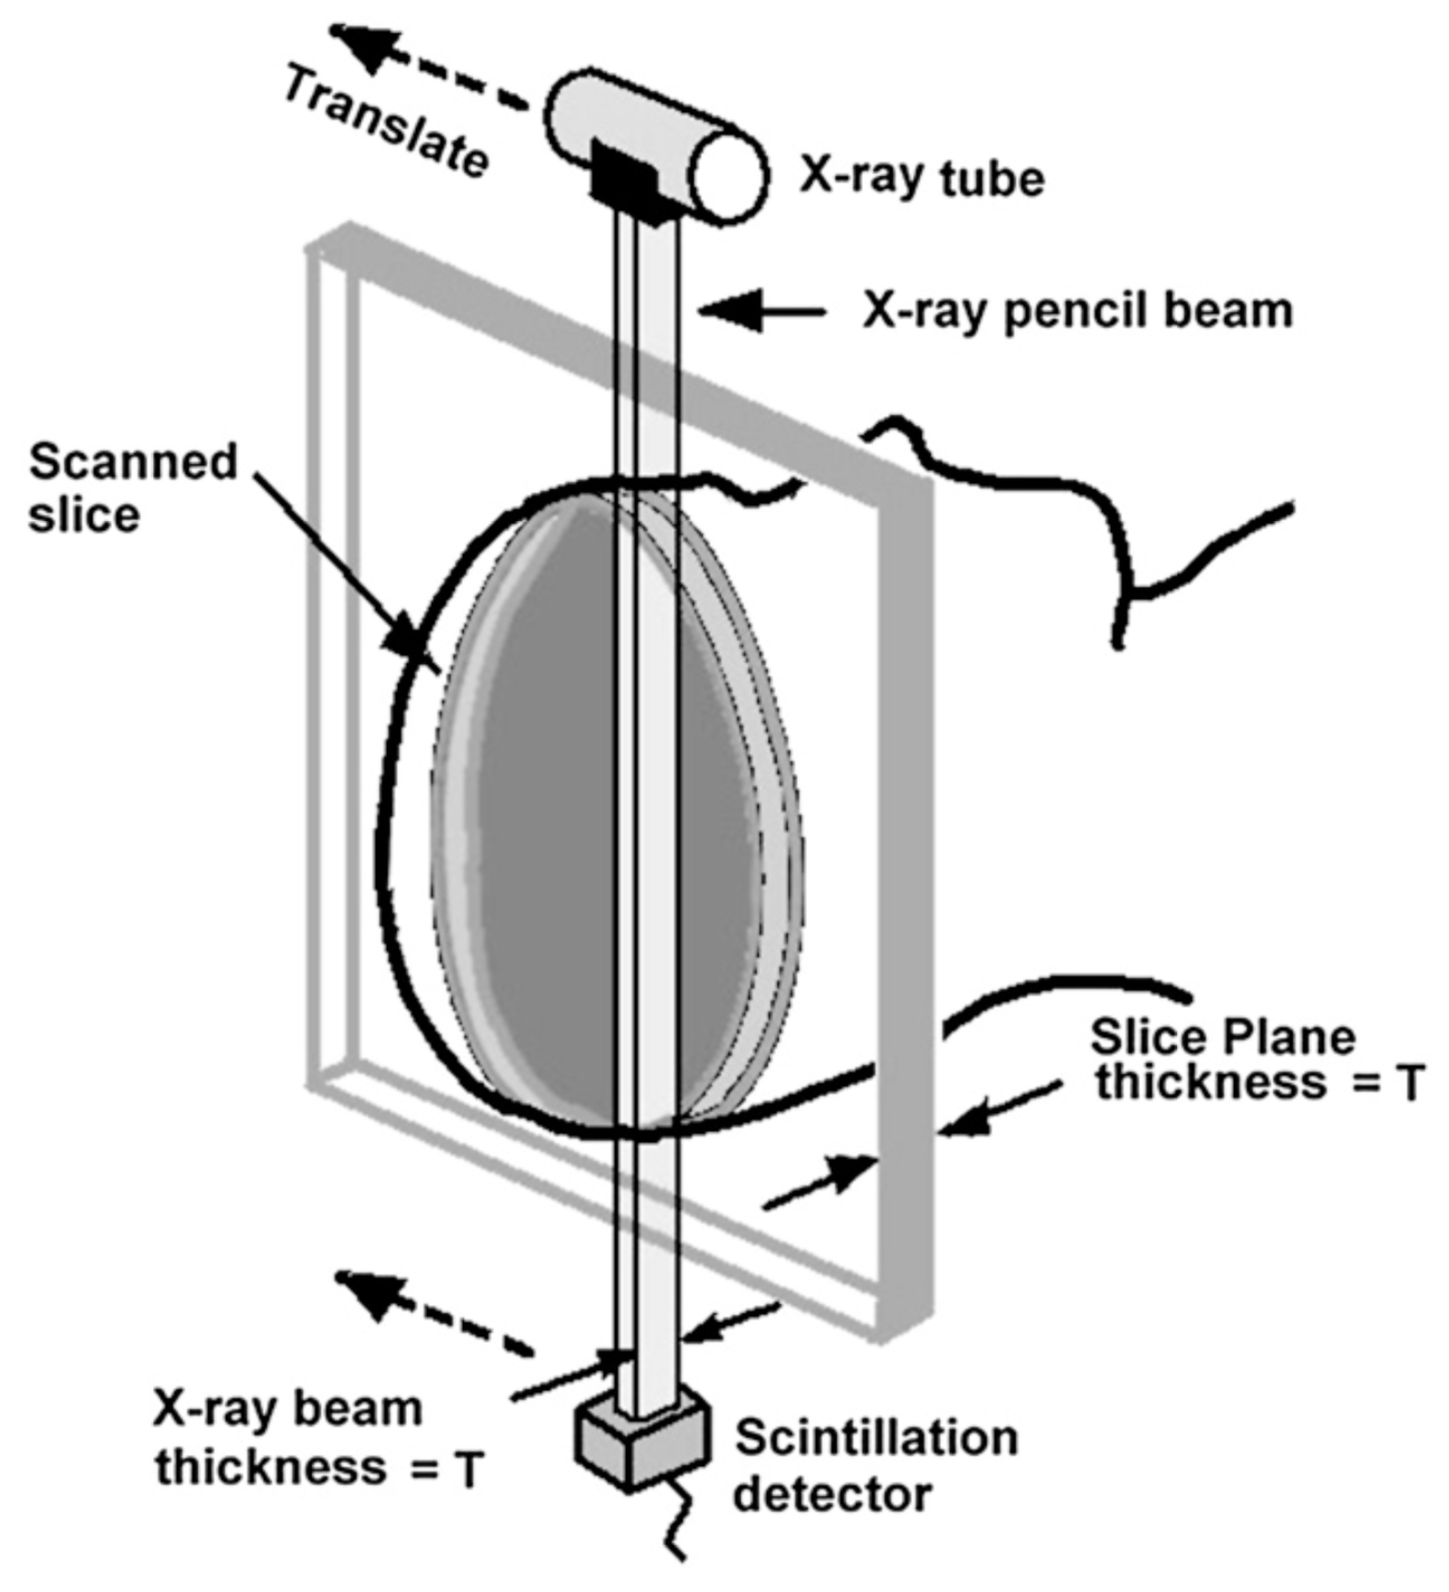
\includegraphics[scale=0.3]{media/0-imaging/ct1.png}
%
\caption{CT arrangement for linear transverse scanning motion of x-ray tube and detector. ~\cite{goldman_2007}}
\label{fig:ct1}
\end{figure}

The x-ray beam path is referred to as a \textit{ray}. The set of rays and measurements made during the the translation is known as a \textit{view}. Several hundred rays are measured in a particular view. The assembly is then rotated about the axis perpendicular to the slice plane by a small increment and a new view is captured. Over a 1000 views are captured as the assembly is rotated through 360$^{\circ}$. Thus, the total number of measurements for a particular slice is the number of rays per view multiplied by the number of views, and is on the order of a million measurement per slice in modern CT machines. See \figref{ct2}.

\begin{figure}[ht]
\centering
		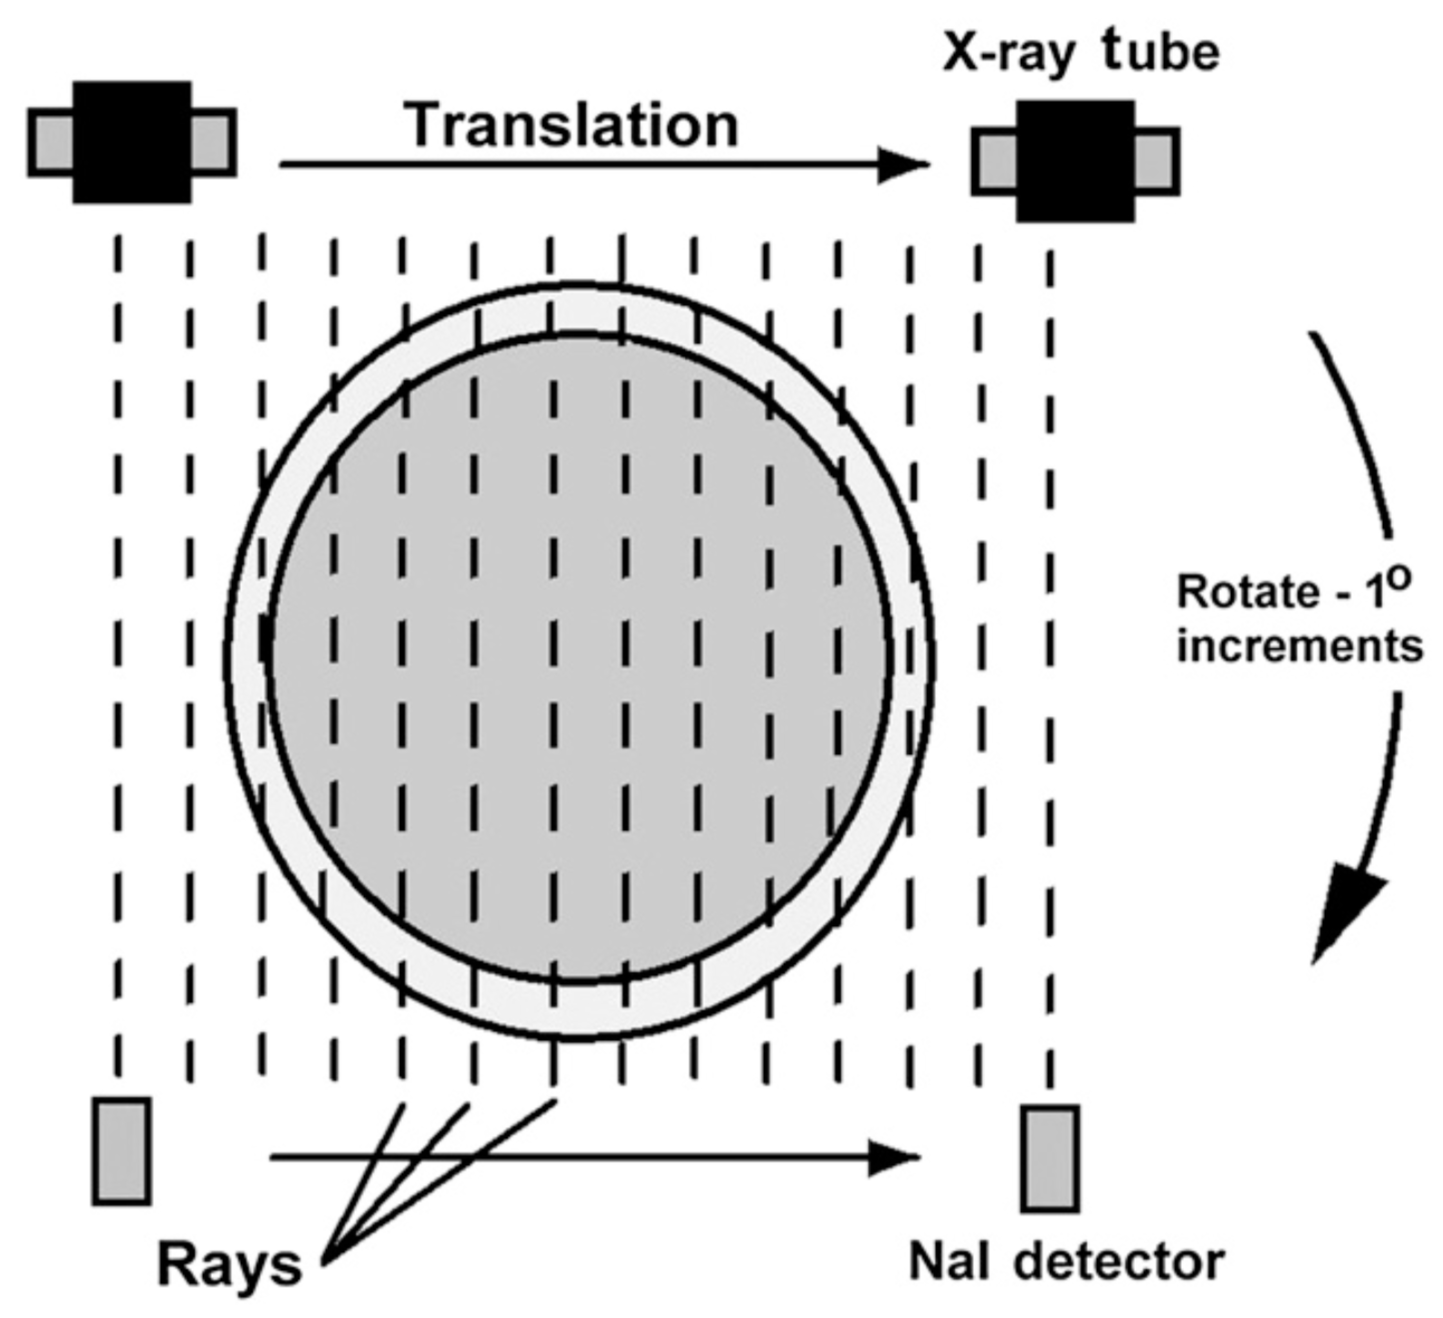
\includegraphics[scale=0.3]{media/0-imaging/ct2.png}
%
\caption{Measurement procedure for first-generation CT. Rays are emitted from the x-ray tube and the attenuated radiation is measured by the detector. The assembly is translated in increments to cover the span of the slice. The process is repeated as the assembly is rotated in increments through 360$^{\circ}$, in this example in 1$^{\circ}$ degree increments~\cite{goldman_2007}}
\label{fig:ct2}
\end{figure}

\textit{Image reconstruction} is the process of deriving the average attenuation coefficient values $f$ for each voxel in a slice from the attenuation measurements made by the x-ray detector. Attenuation increases with the density and atomic number of the tissues in the voxel. Rearranging~\eqnref{init} yields:
\begin{equation}
p(\xi, \theta) = -\ln(I/I_0) = \int\limits_{0}^{L}f(x,y) ds
\end{equation}
The function $p(\xi,\theta)$ is known as the \textit{Radon transform} of the attenuation function $f(x,y)$. The angle $\theta$ corresponds to the angle of rotation of the view, and $\xi$ corresponds to the position along the measured x-ray projection~(\figref{ct3}).

\begin{figure}[ht]
\centering
		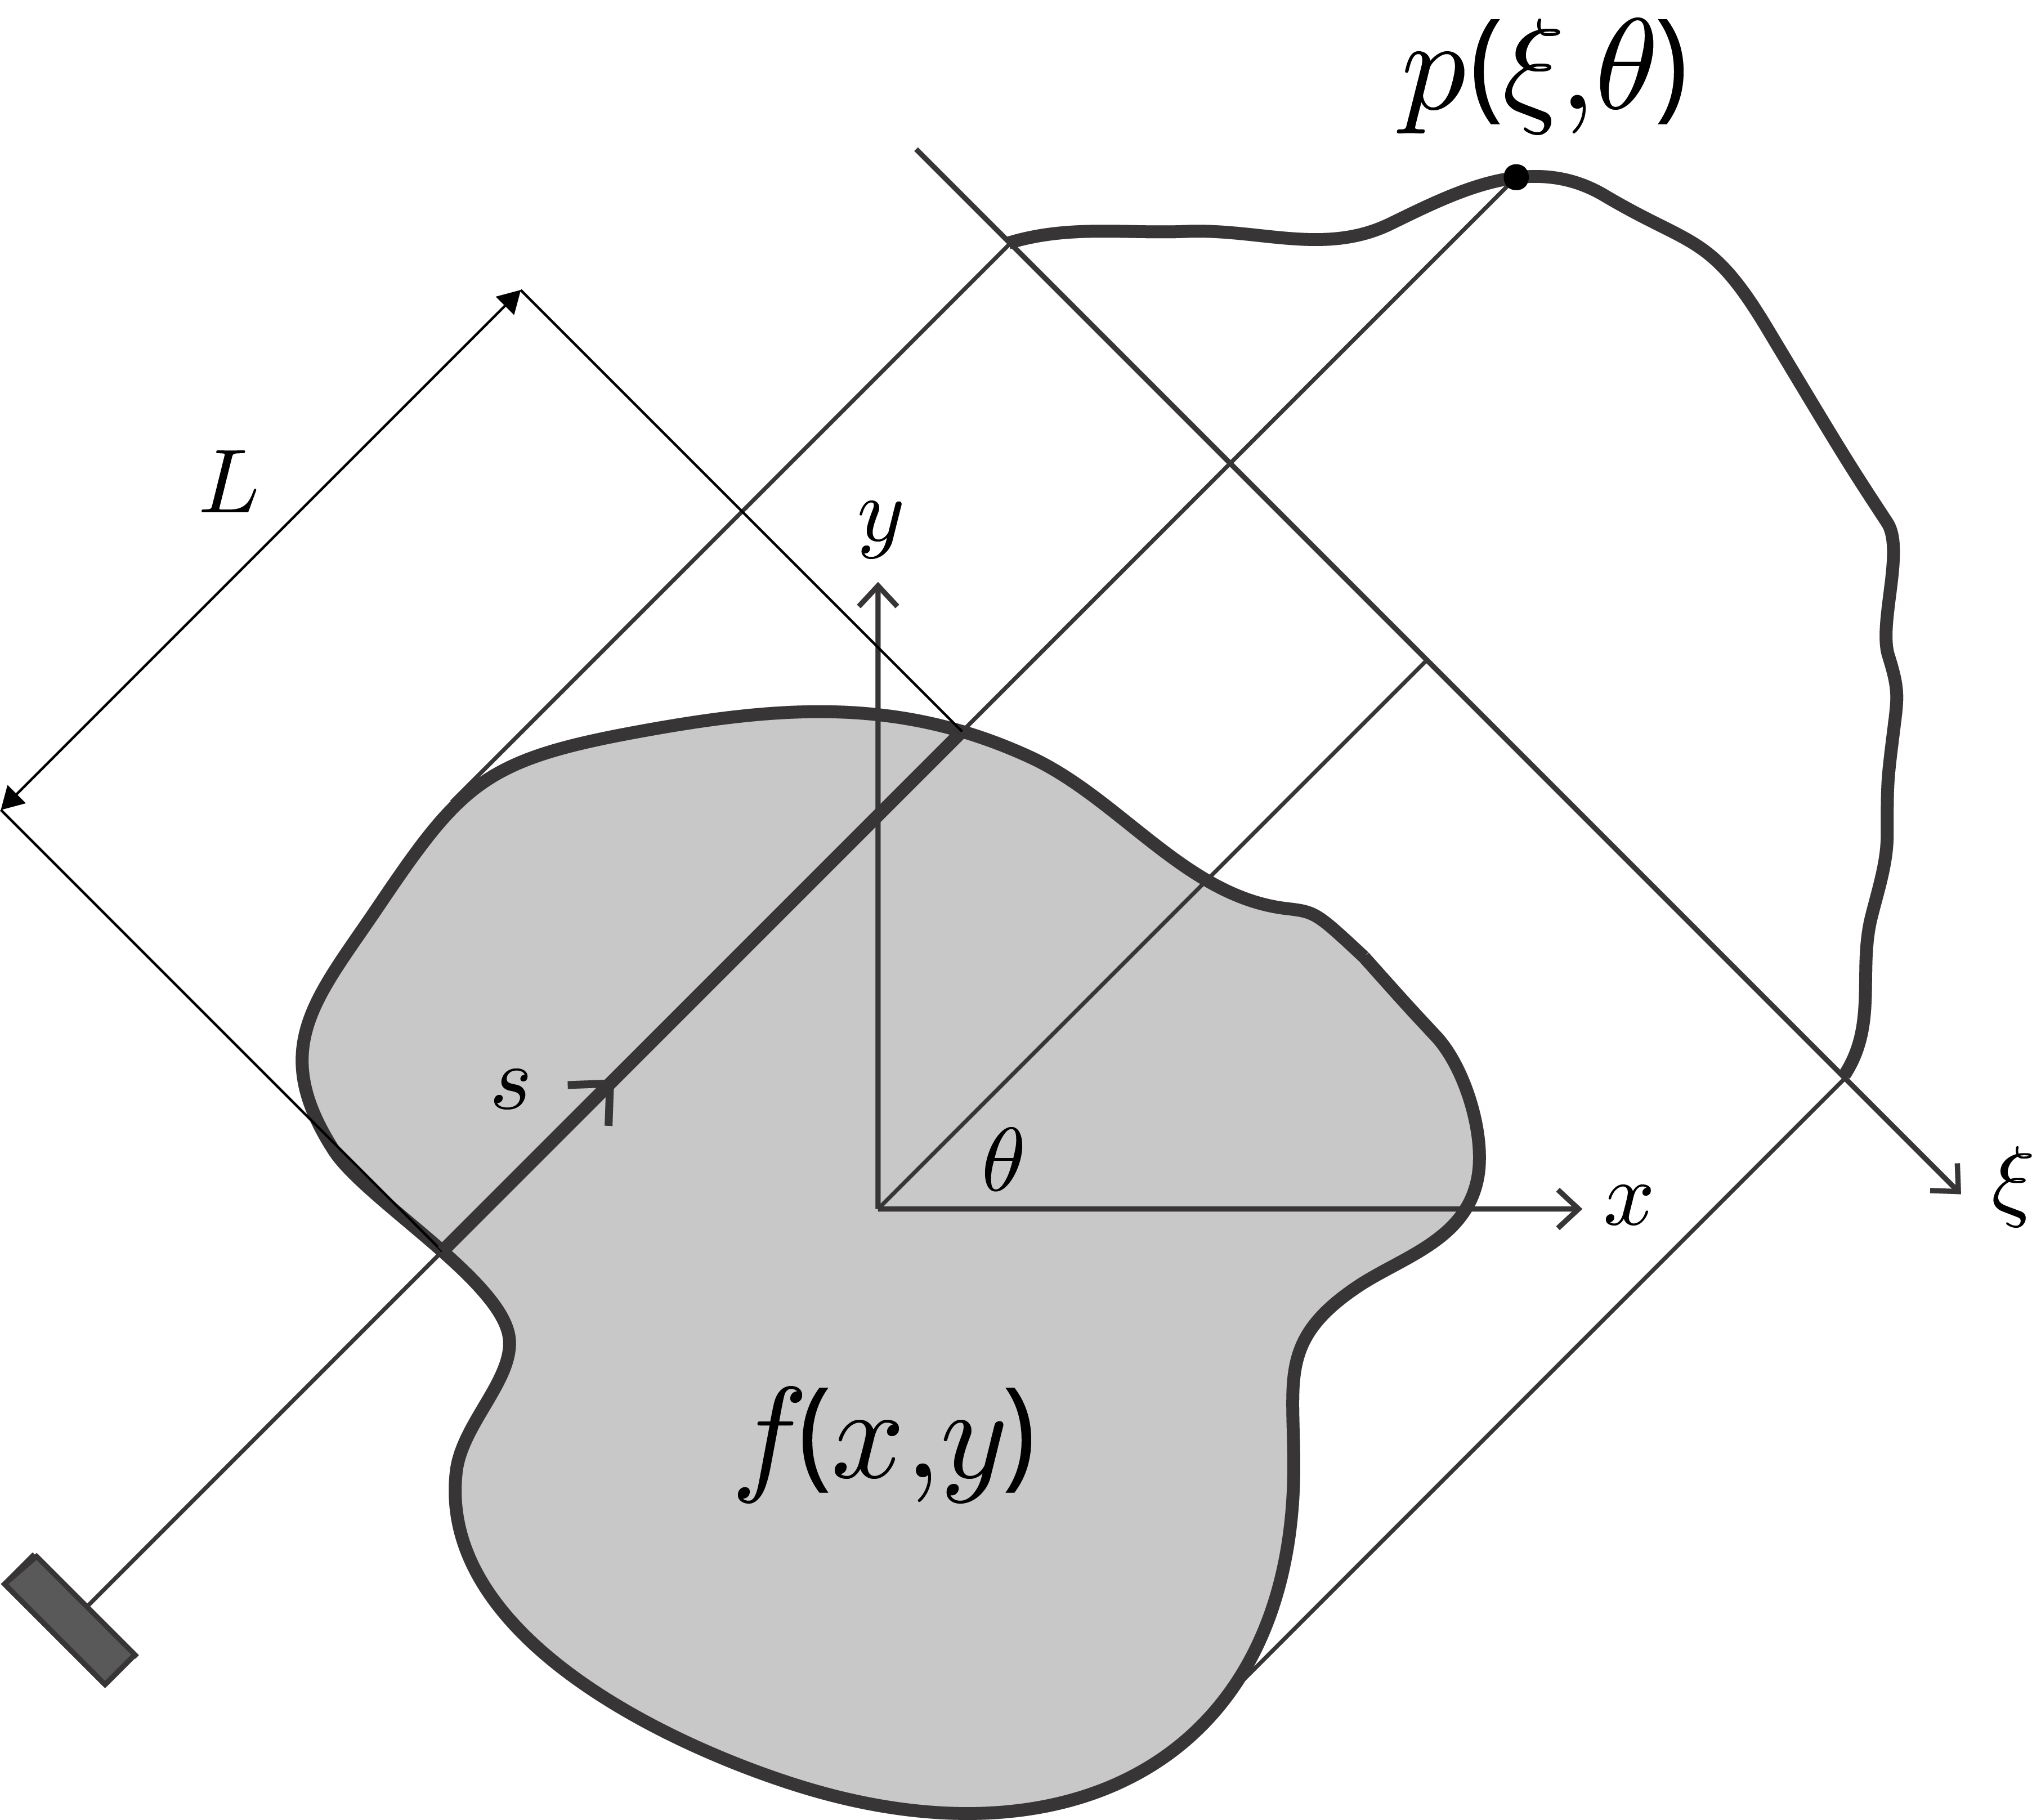
\includegraphics[scale=0.3]{media/0-imaging/ct3.png}
%
\caption{Linear attenuation function $f(x,y)$ for a particular slice, and corresponding projection $p(\xi,\theta)$}
\label{fig:ct3}
\end{figure}

The function $p$ for each $\theta$ view is known as a \textit{projection} of the image $f$. The most popular image reconstruction technique is \textit{backprojection}, in which the function $f$ is backprojected from the projections $p$. Backprojection leads to a blurring of the original image, so the projected images are first filtered prior to backprojection. The technique is known as \textit{filtered backprojection}. It involves computing the Fourier transform of $p$, applying a ramp filter to avoid blurring, computing the inverse Fourier transform of the resulting function, and finally the inverse Radon transform to approximate $f(x,y)$. Filtered backprojection performs best in the presence of a large number of projections, which is the case in modern CT scanners. Please refer to \cite{chetih_2015} for a more detailed description of the procedure.

Finally, the value computed at each voxel is rescaled to produce the \textit{CT number} = $K (f_i - f_w)/f_w$, measured in \textit{Hounsfield units}. The value $f_i$ is the attenuation at a particular voxel, and the value $f_w$ is the attenuation of water. The attenuation coefficient of water is obtained during calibration of the machine. The scaling parameter $K$ is typically a value of 1000 in modern machines.

Improvements in acquisition times, spatial resolution, and image reconstruction times have been made in the last 45 years since the first-generation CT machine was introduced. These improvements mostly involve and increase in x-ray detectors, and more clever arrangements and motions of the x-ray beam and associated detector(s). Detailed descriptions of these improvements can be found in the references cited in this section.

\subsection{Additional Imaging Modalities}
\label{Other Imaging Modalities}

Several other popular imaging modalities exist. The discussion here will be restricted to a brief overview of \textit{ultrasound} (US), as well as some quantitative variations of MRI, CT, and US.

Ultrasound uses high-frequency sound pulses that are emitted from a hand-held ultrasound transducer~\cite{waldman_campbell}. The transducer is applied to the patient's skin through a coupling gel, and sound pulses are reflected back to the transducer from structures within the patient. The magnitude of the reflected sound, or \textit{echo} is converted into a 2D grayscale image. Images are acquired in real-time, and do not require any ionizing radiation. Ultrasound is most commonly used for imaging the abdominal and pelvic regions, as well as imaging the musculoskeletal system. When used to image the heart, ultrasound is referred to as \textit{echocardiography}. Three-dimensional ultrasound techniques have been gaining traction in recent decades, of which there are two varieties for 3D reconstruction: random or \textit{freehand scanning} which is based on free motion of the ultrasound transducer; and \textit{sequential scanning} where the ultrasound motion is predetermined in linear, fan-like or rotational patterns~\cite{valocik_2005, bruining_2000}.

Quantitative versions of the modalities discussed typically attempt to extract material property information in addition to only contrasting different tissues. \textit{Diffusion-tensor imaging} (DTMRI) is used to measure the anisotropy of tissues. Additional magnetic field gradients are applied repeatedly to create images that are sensitized to the diffusion of water in specific directions~\cite{o’donnell_westin_2011}. Least squares is employed to estimate the diffusivity tensor at each voxel. The diffusivity tensor may be used to visualize irregularities in the microstructure of the brain~\cite{alexander_lee_lazar_field_2007}, or to approximate cardiac muscle fiber orientations. \textit{Elastography} is the process of quantitatively imaging the mechanical properties of soft tissues \textit{in vivo}, and is performed using magnetic resonance and ultrasound techniques~\cite{zaleska_2014}. The process involves applying a stress or source of motion that deforms the tissue, imaging the tissue response, and finally processing the data to generate images (\textit{elastograms}) of tissue mechanical properties.~\cite{glaser_manduca_ehman_2012}.\textit{Quantitative computed tomography} (QCT) estimates bone mineral density from CT attenuation data by using a calibration phantom during image acquisition. This information can be used to inform heterogeneous material definitions in computational models of bone~\cite{knowles_2016}.

A more complete review of medical imaging technologies can be found in a number of texts~\cite{suetens_2017, webb_2003}.

\subsection{File Formats}
\label{Data Format-IMG}

Medical images are typically stored as a combination of a short \textit{header} followed by \textit{pixel data}. The header is typically stored in ASCII format and the pixel data is typically binary. They may be found in the same file or in separate ones. Pixel data is often stored either as a set of two-dimensional images representing each slice, or as a single block of information corresponding to the 3D volume. In either case, data is stored as a 1D array, from which the data can be unrolled based on the axis ordering specified in the header. The header provides metadata to allow software to read and store the image based on the pixel data. Namely, the header contains the matrix dimensions, image resolution, image origin, axis order, data type of the pixel data (i.e., unsigned char, int, etc.), endianness of the pixel data, and data compression encoding (e.g., raw, gzip, bzip2). Additional information may be provided as well, including patient data, image acquisition parameters (e.g., MRI pulse sequence), and date of acquisition. On the clinical side, DICOM (Digital Imaging and Communications in Medicine) files are by far the most popular format for storing medical images, due to it's extensive metadata including patient information and image acquisition protocol. On the research side, several formats are available, including MATLAB~\cite{MATLAB}, NRRD (Nearly Raw Raster Data)~\cite{nrrd}, NIfTI (Neuroimaging Informatics Technology Initiative)~\cite{nifti}, and Analyze~\cite{analyzedirect}. These file formats are different flavors of the general format described above. They are geared more towards image post-processing compared to DICOM, by way of less detailed metadata sections.


%%%%%%%%%%%%%%%%%%%%%%%%%%%%%%%%%%%%%%%%%%%%%%%
%%%%%%%%%%%%%%%%%%%%%%%%%%%%%%%%%%%%%%%%%%%%%%%
\section{Image Segmentation Approaches}
\label{Image Segmentation Approaches}

Arguably the most challenging task in the workflow is the subsequent image processing and \textit{segmenting} of the image of interest. \textit{Image segmentation} is the process of ... \figref{seg}. Contrast differences between neighboring tissues can be difficult to identify. \textit{Image processing} involves applying filters to the image to alter voxel intensity values, which can remove noise and emphasize features of the image so as to improve the performance of image segmentation algorithms.

\begin{figure}[ht]
\centering
\subfigure[]{%
		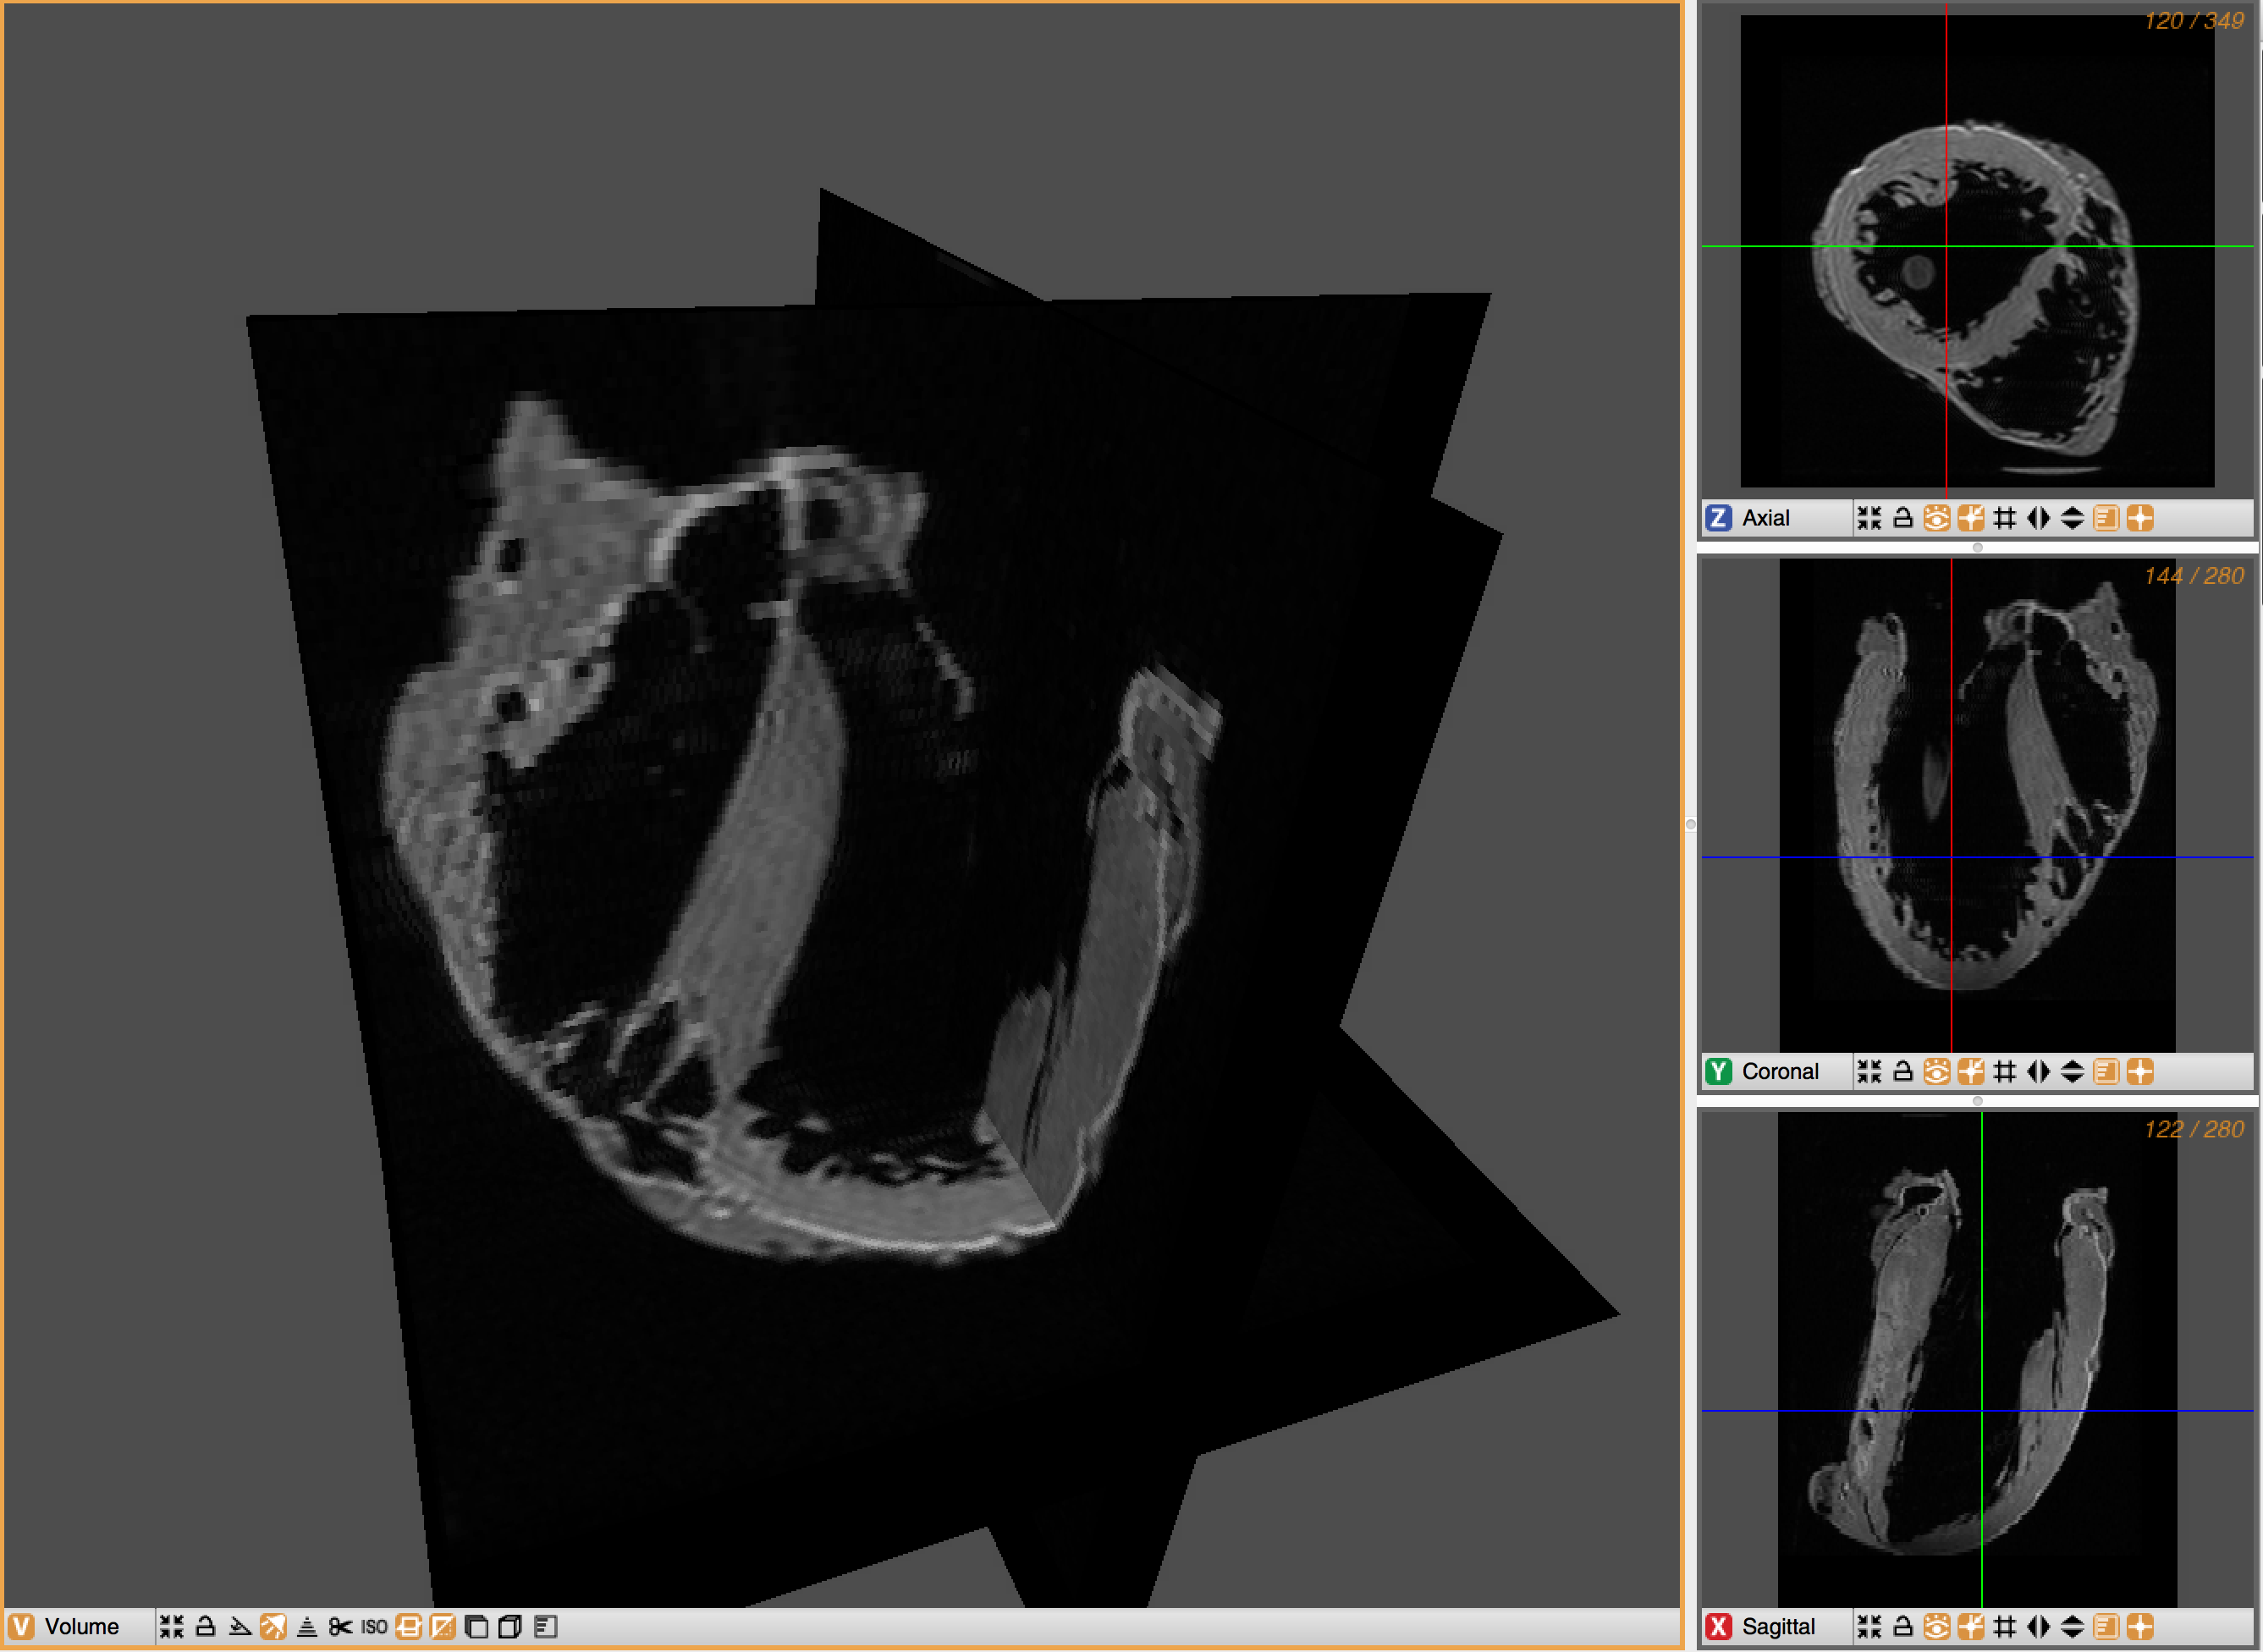
\includegraphics[scale=0.165]{media/1-seg3d/1-raw.png}
\label{fig:seg1}}
\subfigure[]{%
		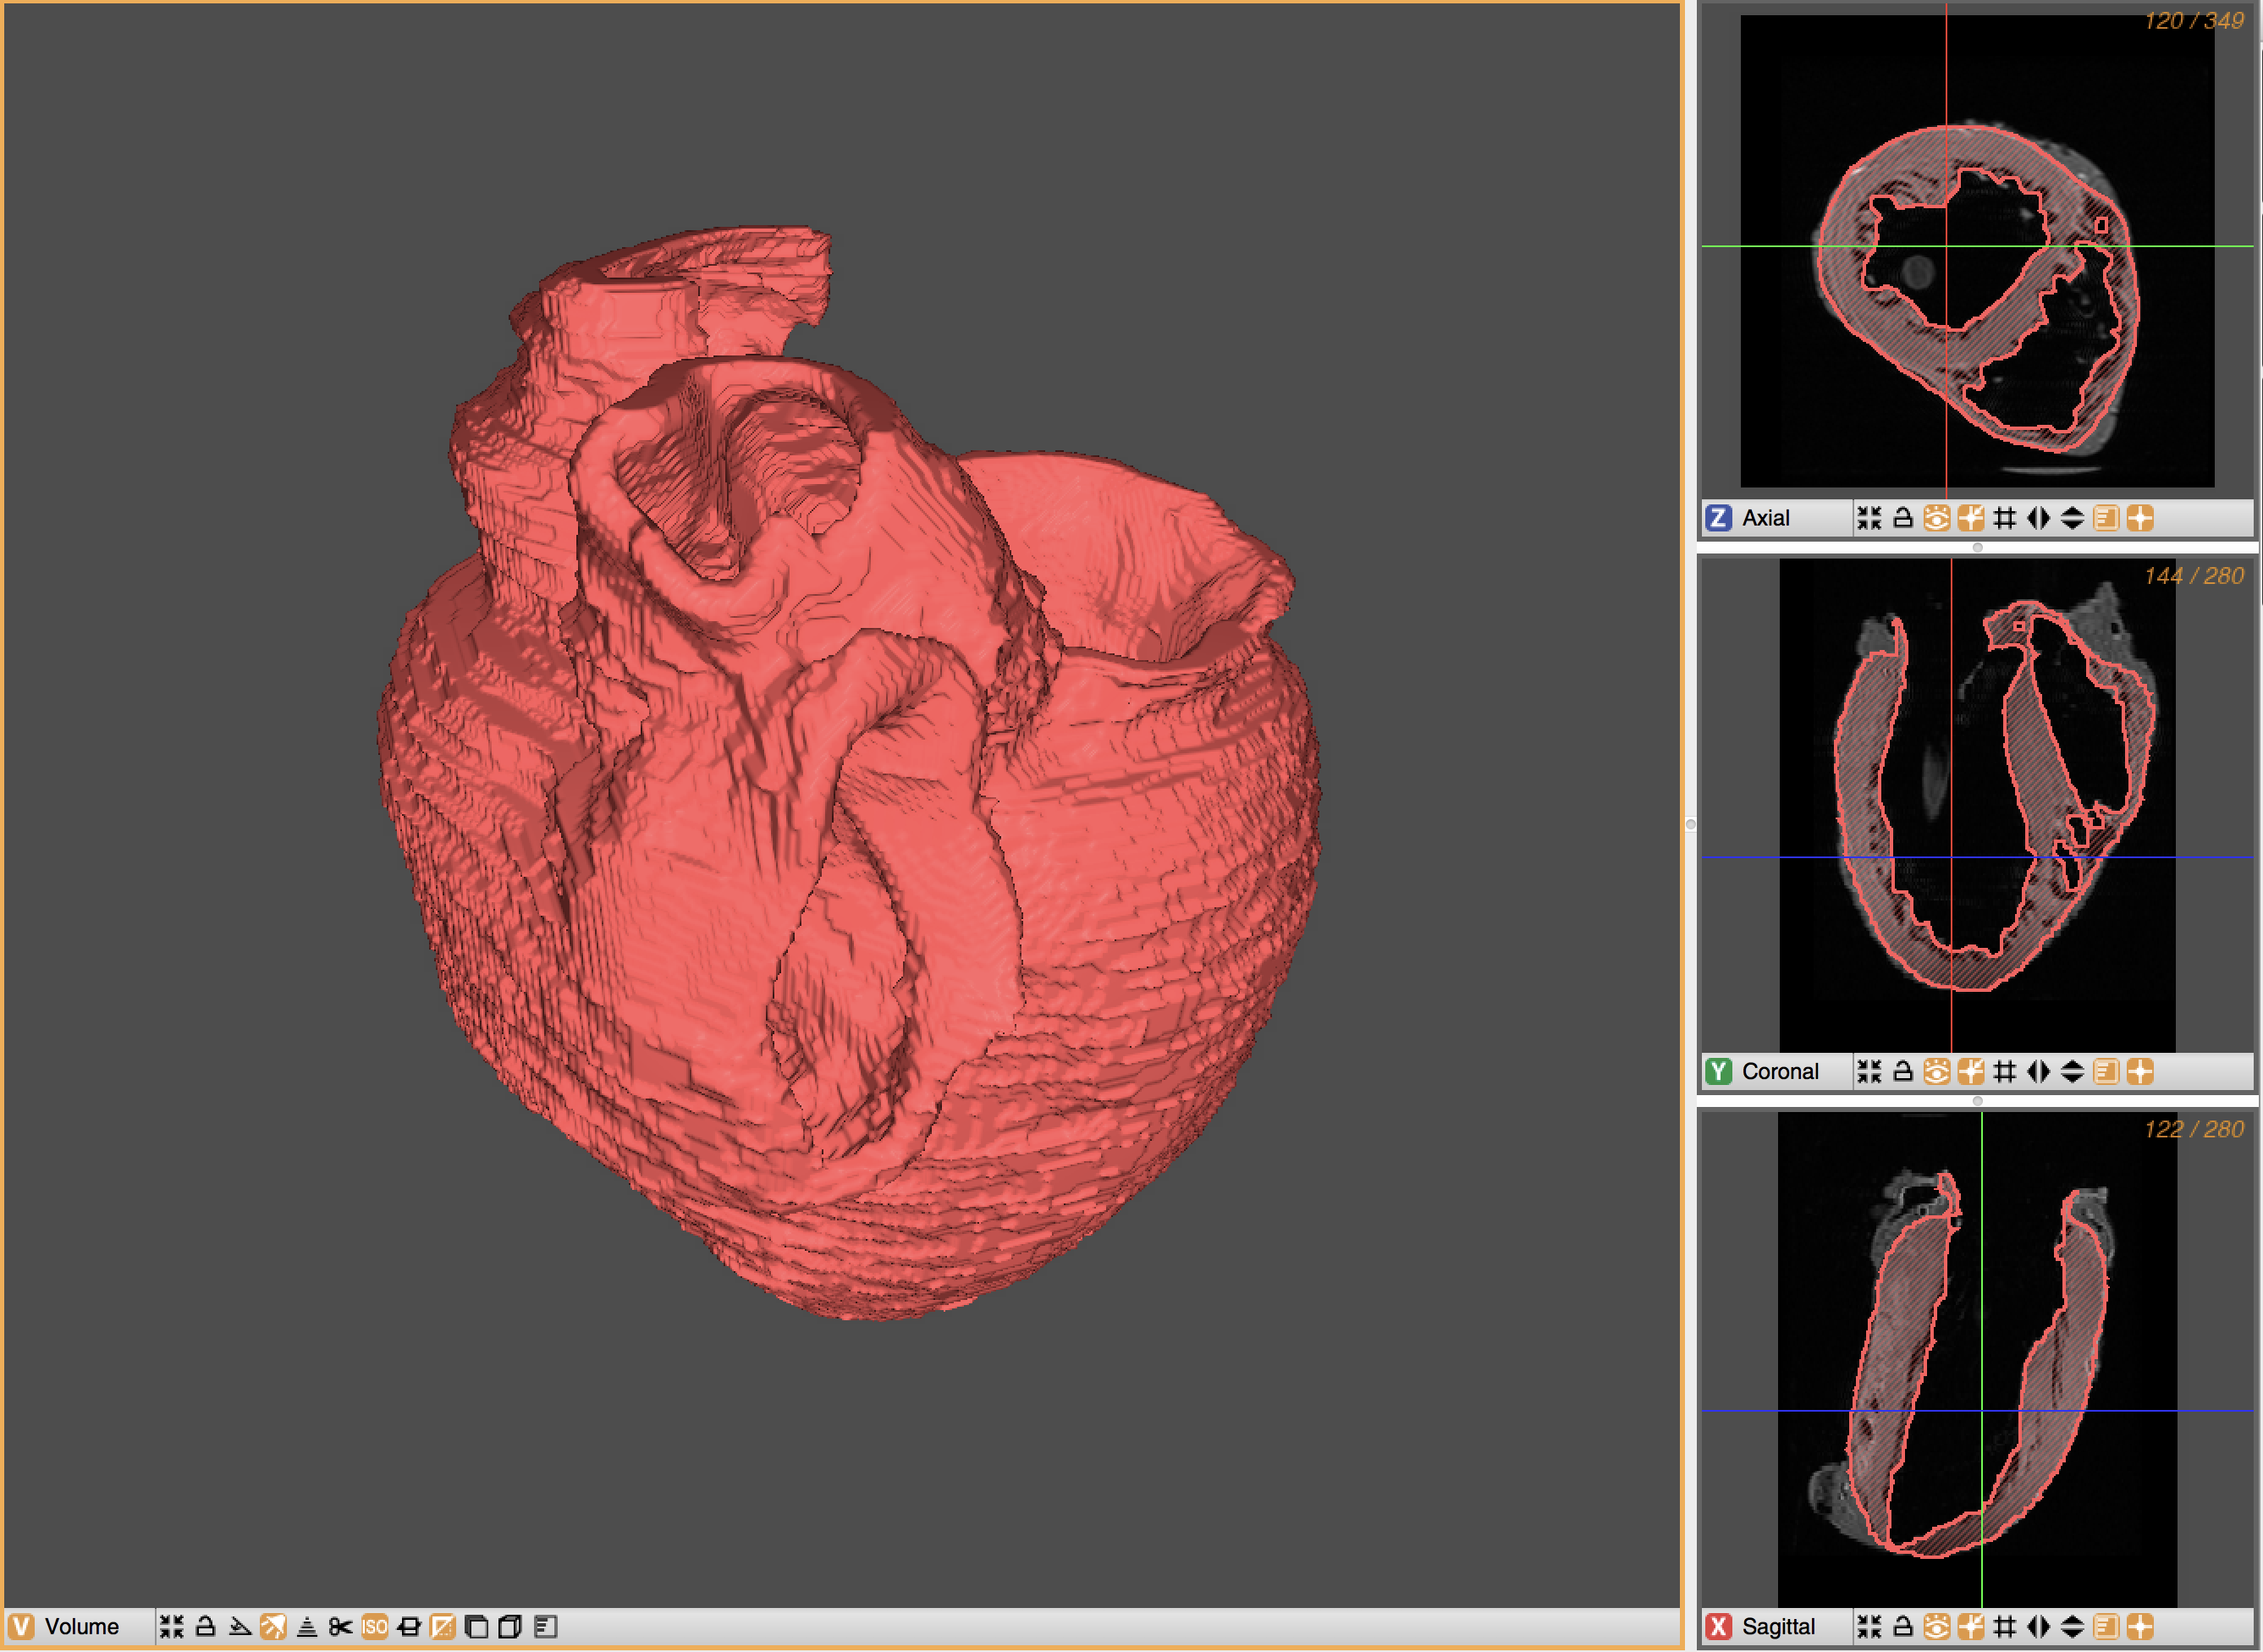
\includegraphics[scale=0.165]{media/1-seg3d/2-seg.png}
\label{fig:seg2}}
%
\caption{(a) MRI of \textit{ex-vivo} human heart, and (b) resulting segmented image mask}
\label{fig:seg}
\end{figure}

The first step in preparing the image data for segmentation is \textit{resampling}. Images most often 

RESAMPLING: for isotropic resolution

Gaussian blur, mean filter, median filter.

\subsection{Review of Image Segmentation Approaches}
\label{Review of Image Segmentation Approaches}

\subsection{Thresholding Methods}
\label{Thresholding Methods}

\subsection{Region-Growing Methods}
\label{Region-Growing Methods}

\subsection{Neural Networks}
\label{Neural Networks}

\subsection{Manual Methods}
\label{Manual Methods}

\subsection{File Formats}
\label{Data Format-SEG}
